%!TEX root = paper.tex
%%%%%%%%%%%%%%%%%%%%%%%%%%%%%%%%%%%%%%%%%%%%%%%%%%%%%%%%%%%%%%%%%%%%%%%%%%%%%%%
%\section{Cloud Gaming Provider Models}

\section{Supply-Side Efficiency Modelling} % OR ONLY: THE SUPPLIER'S PROBLEM
\label{sec:suppliermodelling}



%%%%%%%%%%%%%%%%%%%%%%%%%%%%%%%%%%%%%%%%%%%%%%%%%%%%%%%%%%%%%%%%%%%%%%%%%%%%%%%%
\subsection{Platform Provider Cost Factors}
Backend/Service Requirements and Demands

%%%%%%%%%%%%
\subsubsection{CAPEX}

\begin{itemize}
	\item Regionale Data Center
	\item Gaming Server (GPU-Enabled)
	\item Entwicklungskosten für Software-Plattform(?)
\end{itemize}

\paragraph{Hardware}

\url{https://www.nvidia.com/object/cloud-gaming-gpu-boards.html}
\url{https://www.nvidia.com/object/grid-technology.html}


%%%%%%%%%%%%
\subsubsection{OPEX}

\paragraph{Verkehrsvolumen}

\begin{itemize}
	\item Internetanbindung?
	\item Caching of basic resources is probably not applicable?
\end{itemize}

\paragraph{Serverlaufzeiten}

\begin{itemize}
	\item Energie
	\item Verschleiß
	\item Wartungs- und Betriebspersonal oder Anmietung
	\item Frage: Rechnet sich Anmietung von Ressourcen bei großen generischen Rechenzentren? Annahme nein, da man selbst ein großer Anbieter wäre u. die Margin wegfallen. Auf der anderen Seite gibt es Hardware die für Games im Serverbereich besser skalieren? Wenn ja, kann umso mehr kein generischer Anbieter die Lösung sein
\end{itemize}

\paragraph{Spiele-Lizenzen und -Adaptionskosten (?)}
Modelannahme: Kosten pro Nutzung (realistisch eher in Blöcken verrechnet)



%%%%%%%%%%%%%%%%%%%%%%%%%%%%%%%%%%%%%%%%%%%%%%%%%%%%%%%%%%%%%%%%%%%%%%%%%%%%%%%

%\subsection{Computational Efficiency}

Based on the collected consumer price figures of Section XXX, this section will elaborate on the required computational efficiency, i.e., cost per hosted subscriber, in order to successfully establish cloud gaming approaches on the market. Due to the limited available data, this investigation will follow a one data center assumption. Due to the demands of cloud gaming to serve both high performance and low latency, regional data centers will play a dominant role in the provider side cost modelling. Following this assumption, hereinafter a specific model is created that characterises at which cost efficiency levels the cloud gaming business can be operated successfully.

\begin{figure}[!t]
	\centering
	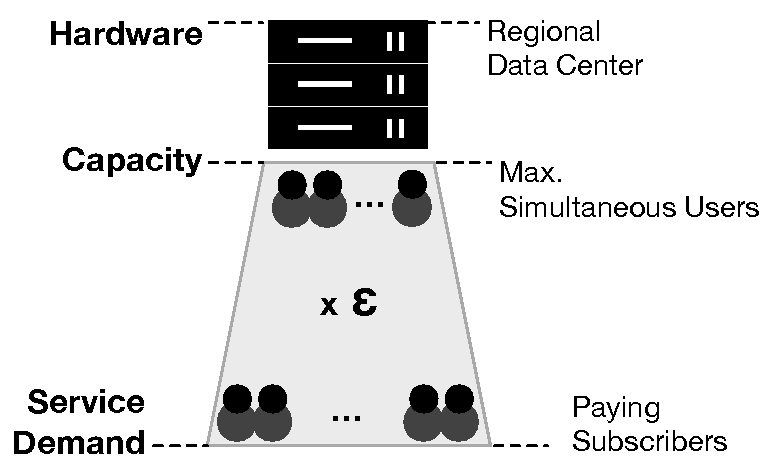
\includegraphics[width=0.65\columnwidth]{images/overbooking_datacenter.pdf}
	\caption{Overbooking of available computational capacity.}
\label{fig:overbooking_datacenter}
\end{figure}

The computational efficiency considers the maximum overbooking rate $\epsilon \geq 1$, where $\epsilon = 1$ refers to no overbooking. Due to expected peaky demand curve, the overbooking rate $\epsilon$, as inverse of the capacity load $\rho$, is derived from the peak demand $L$ (simultaneously connected users) and the available data center capacity $Cap$ (number of users that can be handled),

\begin{align}
	\rho :=& \frac{\lambda}{\mu} = \frac{L}{Cap} \quad, \\
	\epsilon :=& \frac{1}{\rho} \quad.
	%\frac{Cap}{d_{peak}} \quad ,
	%\epsilon = \frac{1/rho} = 
\end{align}

LAMBDA 
MU ERKLAEREN

This modelling stands in contrast to the classical formulation of Little's law, which focuses on long-term averages. The maximum number of subscribers $d$ (maximum service demand) is, thus, given by

\begin{equation}
	 d = Cap \cdot \epsilon \quad .
\end{equation}

The average monthly customer price $\bar{p}$ aggregates the monthly subscription fee and the customer's depreciation costs for the hardware investments on a four years investment duration. We further consider a minimum profit margin $m$ of $3 \%$, which is in line with the average figure for the global game industry\footnote{\url{http://www.polygon.com/2012/10/1/3439738/the-state-of-games-state-of-aaa}} and substantially below the cloud computing figures that can range up to $16.9\%$\footnote{\url{http://www.forbes.com/sites/georgeanders/2015/04/23/amazons-web-services-delight-16-9-margins-more-joy-ahead/\#73324aa64b4e}} and potentially even higher\footnote{\url{http://www.bloomberg.com/news/articles/2015-12-02/microsoft-should-disclose-cloud-revenue-margins-ballmer-says}}.

%Global Games statistics / billion revenues 2012-2016: http://newzoo.com/infographics/global-games-market-report-infographics-2013/
% Game industry = 3%: http://www.polygon.com/2012/10/1/3439738/the-state-of-games-state-of-aaa
% Game industry in the past (2009 – average console game with margin of 40%): http://www.businessinsider.com/casual-gaming-profit-margins-near-90-2009-10?IR=T
% Profit margins in cloud computing:
%	Amazon 16.9% (2015): http://www.forbes.com/sites/georgeanders/2015/04/23/amazons-web-services-delight-16-9-margins-more-joy-ahead/#73324aa64b4e
% 	Microsoft 44% (2015) -- questionable: http://www.bloomberg.com/news/articles/2015-12-02/microsoft-should-disclose-cloud-revenue-margins-ballmer-says

\begin{align} \label{eq:computational_efficiency}
	\frac{\epsilon \cdot Cap \cdot \bar{p}}{Cap} :=& \underbrace{\frac{\mathcal{C}_{cap}}{Cap}}_{\mathcal{C}_{u}} \cdot m\\
	%= C_{u} = \frac{C_{cap}}{Cap} :=& \frac{\epsilon \cdot \bar{p}}{m}
	\Longrightarrow \mathcal{C}_{u} :=& \frac{\epsilon \cdot \bar{p}}{m}
\end{align}

When treating the costs of the regional data center as blackbox (operational and capital costs for the data center, and required game licensing fees), the analysis can concentrate on the required capacity and licensing cost $\mathcal{C}_{u}$ per connected user $u$.

%\begin{equation}
%	ce = \frac{C_{cap}}{Cap} \quad .
%\end{equation}

%%%%%%%%%%%%%%%%%%%%%%%%%%%%%%%%%%%%%%%%%%%%%%%%%%%%%%%%%%%%
%SOME DATA CONSIDERATIONS:


% ALTE DATEN:
% Anderer Messpunkt:
% Höchststand (simultaneous): 12 406 722 Nutzer maximal, Feb 13 - Feb 15
% Peak immer abends. Niedrigster Wert bei <7.5 Mio Nutzern
% => \epsilon von 75/12,406722 = 6,0451100621
% Eigentlich, da steam wächst, > 6 eine gute Annahme. Wir könnten versuchen Schranken zu definieren.
% Wenn wir annehmen, dass Skalierung gut funktioniert, benoetigen wir keinen Buffer. Sollen wir Buffer verwenden?

% NEUE DATEN:
% ANGLE 1:
%According to http://venturebeat.com/2014/01/15/steam-has-75-million-registered-users-third-party-steam-controllers-and-other-tidbits-from-valves-dev-days/
% Customer base of Steam was 75 Million active users in 2014. 
% %Vermutlich Nutzerzahl mittlerweile hoeher. Schaetzungen waeren also konservativ ausgerichtet.
%According to http://store.steampowered.com/stats/?l=german
% Testzeitraum: Feb 16 – 18
% Höchststand (simultaneous): 11 645 185	 Nutzer maximal
%	-> Anteil Grundgesamtheit: 0.1552691333
%	-> Epsilon: 6.4404301005 (75/11,645185)
% Tiefststand (simultaneous): 6 527 571 
%	-> Relatives Wachstum: 1.7839997451 = 78%

% ANGLE 2: 
% Data from ``Enabling Experiments for Energy-Efficient Data Center Networks on OpenFlow-based Platform''
% Data is on server loads for video traffic (Video on Demand) of a big ISP in Vietnam
% Does not give indications on parent population. So, we will compare the steam data with this data in a relativ fashion.
% Thursday values in Fig 2. are most peaky. So we take them.
% Höchststand: 71.190% at 17.530 (da time. Half past 5)
% Tiefststand: 7.971 % at 7.88 (day time time. Almost 8 o'clock – nobody watches video)
% 	-> Relatives Wachstum: 8.9311253293 = 893.1%
% Umgelegt vom Mindesstand bei Steam waere das dann:
%	6 527 571 * 8.9311253293 = 58.298.554,697 (geringfuegig verschoeben zu den initialen Daten%

%%%%%%%%%%%%%%%%%%%%%%%%%%%%%%%%%%%%%%%%%%%%%%%%%%%%%%%%%%%%

\todo[inline]{NOW LET'S ADD THE DATA. Check the 12.4m. E.g. user older data. Introduce customer base data and reasoning above. Illustrate that epsilon will be around 6.}

When considering a measurement iteration between Feb 16 and 18, the minimum and maximum number of simultaneously connected users\footnote{\url{http://store.steampowered.com/stats/}, accessed: Feb 18, 2016} is 6.53m and 11.65m	 resp. Setting the maximum in relationship with the 75 million active steam users\footnote{http://venturebeat.com/2014/01/15/steam-has-75-million-registered-users-third-party-steam-controllers-and-other-tidbits-from-valves-dev-days/, last accessed: Feb 18, 2016}, we can calculate an $\epsilon_{max}$ of $6.44$. For crossvalidation purposes, link load considerations for other media streaming services may also be considered: When comparing the relative load level change between the minimum and maximum utilisation of a large Vietnamese ISP's Video on Demand (VoD) streaming server as given in \cite{thanh2012enabling} (reconstructed data for Thursday in Fig 2. as most peaky day), with the comparable change in the case, we would obtain a maximum number of simultaneously connected users of 58.3 million and an $\epsilon_{min}$ of $1.2931034483$. While the discrepancy may appear high, the associated payment modalities may be at cause: While steam sells game licenses, VoD services often use a subscription services (a flat rate for a given time period). For the subsequent analysis we will consider the range between the minimum $\epsilon_{min}$ and maximum $\epsilon_{max}$.

As a result, the capacity and licensing cost per user $\mathcal{C}_u$ needs to be below XXXXXXXX (for $\epsilon_{max}$)  or XXXX Euro ($\epsilon_{min}$) for obtaining the required minimum margin $m$. Scaling theses costs to the population of $11.65m$ and  $58.3m$ users, we obtain a total server capacity cost $\mathcal{C}_{Cap}$, which should not exceed XXX and XXX Euro resp. 

%Thus, we can characterise that the successful cloud game provider will have a maximum $C_{u}$ in the following bounds:
% for a successful market operation.




Due to the requirement of using special hardware that is focused on the gaming use case, hardware sharing with other cloud applications seems unrealistic. Thus $\mathcal{C}_u$ can hardly be reduced by cloud service collaboration. However, to lower the investment demands, the platform operator could aim at increasing the overbooking ratio $\epsilon_{min}$ for the subscription case closer to the $\epsilon_{max}$ of the classical purchasing model. The could provider could, for example, offer off-peak subscriptions that allow the access to the platform only outside of peak hours.

%by deploying subscription models that foster the off-peak usage, i.e., off-peak subscriptions that allow the access to the platform only outside of peak hours. This may allow a convergence of $C_u$ for subscription-based charging models close to $\epsilon_{max}$.

%When considering a substantial increase of the $\epsilon$ to $8$---the realistic maximum when considering the high peak time centricity of the gaming use case---, we obtain a substantially lowered $C_{u}$ requirement of $6.44$. 

%\todo[inline]{ADD DATA}

This maximum does not consider that the operator may not be able to fully utilize the available capacity or may not hold the optimal game licenses at all times. Thus, in practice, we recommend target $\mathcal{C}_{u}$ values to be lower than the calculate values.

\todo[inline]{NOW LET'S INTERPRET IF THAT SOUNDS LIKE A HARD THING TO DO OR NOT. AND THERE WE GO.}



